\documentclass[10pt,a4paper]{article}

\usepackage[utf8]{inputenc}
\usepackage[T1]{fontenc}
\usepackage{lmodern}
\renewcommand{\familydefault}{\sfdefault}
\usepackage{amsmath,amssymb}
\usepackage{geometry}
\usepackage{graphicx}
\usepackage{xcolor}
\usepackage{tikz}
\usetikzlibrary{shapes.geometric,calc,positioning}
\usepackage{fancyhdr}
\usepackage{hyperref}
\usepackage{array}
\usepackage{booktabs}
\usepackage{colortbl}

\geometry{
  a4paper,
  top=0.48in,
  bottom=0.48in,
  left=0.52in,
  right=0.52in,
  headheight=16pt,
  headsep=6pt,
  footskip=16pt
}

\setlength{\parindent}{0pt}
\setlength{\parskip}{2.2pt}

% --- Color Palette (Magazine / Project Delphi Style) ---
\definecolor{navybg}{HTML}{0B1325}
\definecolor{panelbg}{HTML}{0F172A}
\definecolor{slateink}{HTML}{1E293B}
\definecolor{mutedink}{HTML}{475569}

\definecolor{sky}{HTML}{0284C7}
\definecolor{skylight}{HTML}{E0F2FE}
\definecolor{skyborder}{HTML}{38BDF8}

\definecolor{emerald}{HTML}{15803D}
\definecolor{emeraldlight}{HTML}{DCFCE7}
\definecolor{emeraldborder}{HTML}{4ADE80}

\definecolor{amber}{HTML}{B45309}
\definecolor{amberlight}{HTML}{FEF3C7}
\definecolor{amberborder}{HTML}{F59E0B}

\definecolor{crimson}{HTML}{B91C1C}
\definecolor{crimsonlight}{HTML}{FEE2E2}
\definecolor{crimsonborder}{HTML}{F87171}

\definecolor{purple}{HTML}{6D28D9}
\definecolor{purplelight}{HTML}{F3E8FF}
\definecolor{purpleborder}{HTML}{A78BFA}

\definecolor{goldaccent}{HTML}{FACC15}
\definecolor{cyanaccent}{HTML}{38BDF8}
\definecolor{softgray}{HTML}{F8FAFC}
\definecolor{cardgray}{HTML}{F1F5F9}

\hypersetup{
  colorlinks=true,
  linkcolor=sky,
  citecolor=sky,
  urlcolor=sky,
  pdftitle={Methods, Models, Knowledge-Graph Queries & Code Provenance: D'Arcy Thompson (1917) Study — By Joel Dietz},
  pdfauthor={Joel Dietz (Project Delphi)}
}

% --- Inline Pill Badge ---
\newcommand{\pillbadge}[2]{%
  \tikz[baseline=(char.base)]{%
    \node[
      shape=rectangle,
      rounded corners=2.5pt,
      fill=#1,
      text=white,
      inner xsep=4.5pt,
      inner ysep=1.5pt,
      font=\sffamily\bfseries\scriptsize
    ] (char) {#2};%
  }%
}

% --- Magazine Section Header Banner ---
\newcommand{\prettysection}[3]{%
  \vspace{2.5pt}%
  \noindent
  \begin{tikzpicture}
    \node[
      rectangle,
      rounded corners=4.5pt,
      fill=#2!10,
      draw=#2!65,
      line width=0.95pt,
      inner xsep=9pt,
      inner ysep=4.5pt,
      text width=\dimexpr\textwidth-20pt\relax,
      align=left
    ] (secbox) {%
      \tikz[baseline=(n.base)]{
        \node[circle, fill=#2, text=white, inner sep=2.2pt, font=\sffamily\bfseries\footnotesize] (n) {#1};
      }%
      \hspace{5pt}{\sffamily\bfseries\normalsize\color{navybg}#3}%
    };
    \fill[#2, rounded corners=1.5pt] (secbox.south west) rectangle ([xshift=3.8pt]secbox.north west);
  \end{tikzpicture}%
  \vspace{1pt}\par
}

% --- Styled Callout Card ---
\newcommand{\calloutcard}[5]{%
  \noindent
  \begin{tikzpicture}
    \node[
      rectangle,
      rounded corners=5pt,
      fill=#2,
      draw=#1!65,
      line width=1.0pt,
      inner xsep=9.5pt,
      inner ysep=6pt,
      text width=\dimexpr\textwidth-21pt\relax,
      align=left
    ] (card) {%
      {\sffamily\bfseries\scriptsize\tikz[baseline=(b.base)]{\node[rounded corners=2.5pt,fill=#1,text=white,inner xsep=5pt,inner ysep=1.5pt](b){#3};}}%
      \hspace{5pt}{\sffamily\bfseries\small\color{navybg}#4}\\[2.5pt]
      {\small\color{slateink}#5}%
    };
    \fill[#1, rounded corners=1.5pt] (card.south west) rectangle ([xshift=4pt]card.north west);
  \end{tikzpicture}\par
}

% --- Dark Framed Figure Card ---
\newcommand{\prettyfigure}[4]{%
  \noindent
  \begin{tikzpicture}
    \node[
      rectangle,
      rounded corners=6pt,
      fill=navybg,
      draw=cyanaccent!80,
      line width=1.0pt,
      inner sep=5.5pt,
      text width=\dimexpr\textwidth-13.5pt\relax,
      align=center
    ] (figcard) {%
      \includegraphics[width=0.985\textwidth,height=#1,keepaspectratio]{#2}\\[2.5pt]
      \begin{minipage}{0.96\textwidth}
        \raggedright
        {\sffamily\bfseries\scriptsize\color{goldaccent}#3}\hspace{3pt}%
        {\sffamily\scriptsize\color{white!92!black}#4}%
      \end{minipage}
    };
  \end{tikzpicture}\par
}

% --- Header & Footer ---
\pagestyle{fancy}
\fancyhf{}
\renewcommand{\headrulewidth}{0pt}
\fancyhead[L]{%
  \tikz[baseline=(h.base)]{
    \node[rounded corners=2pt, fill=navybg, text=goldaccent, inner xsep=5pt, inner ysep=1.8pt, font=\sffamily\bfseries\scriptsize] (h) {METHODS \& PROVENANCE};
  }\hspace{4pt}{\sffamily\scriptsize\color{mutedink}D'Arcy Thompson (1917) Study $\cdot$ Models, Knowledge-Graph Queries \& Repository Code Reuse}
}
\fancyhead[R]{{\sffamily\bfseries\scriptsize\color{sky}Joel Dietz $\cdot$ Project Delphi}}
\fancyfoot[L]{{\sffamily\scriptsize\color{mutedink}\texttt{github.com/fractastical/morpholib} $\cdot$ \texttt{github.com/fractastical/project-delphi-loop} $\cdot$ \texttt{docs/THOMPSON\_METHODS.md}}}
\fancyfoot[R]{%
  \tikz[baseline=(p.base)]{
    \node[rounded corners=2pt, fill=sky, text=white, inner xsep=6pt, inner ysep=1.8pt, font=\sffamily\bfseries\scriptsize] (p) {Page \thepage\ of 5};
  }
}

\begin{document}

% ============================================================================
% PAGE 1: HERO BANNER + AI/LLM AGENT ARCHITECTURE + MATHEMATICAL MODELS
% ============================================================================
\noindent
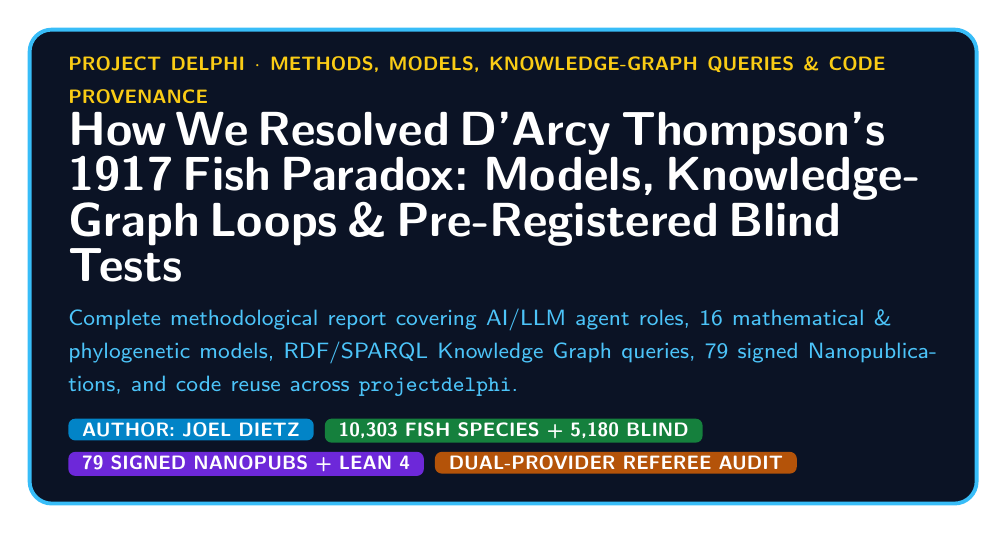
\begin{tikzpicture}
  \node[
    rectangle,
    rounded corners=8pt,
    fill=navybg,
    draw=cyanaccent,
    line width=1.4pt,
    inner xsep=14pt,
    inner ysep=10pt,
    text width=\dimexpr\textwidth-30.8pt\relax
  ] (hero) {%
    {\sffamily\bfseries\scriptsize\color{goldaccent}PROJECT DELPHI $\cdot$ METHODS, MODELS, KNOWLEDGE-GRAPH QUERIES \& CODE PROVENANCE}\\[3pt]
    {\sffamily\bfseries\fontsize{16.5}{19.5}\selectfont\color{white}How We Resolved D'Arcy Thompson's 1917 Fish Paradox: Models, Knowledge-Graph Loops \& Pre-Registered Blind Tests}\\[4pt]
    {\sffamily\footnotesize\color{cyanaccent!90!white}Complete methodological report covering AI/LLM agent roles, 16 mathematical \& phylogenetic models, RDF/SPARQL Knowledge Graph queries, 79 signed Nanopublications, and code reuse across \texttt{projectdelphi}.}\\[4pt]
    \tikz[baseline=(a.base)]{\node[rounded corners=2.5pt,fill=sky,text=white,inner xsep=5pt,inner ysep=1.5pt,font=\sffamily\bfseries\scriptsize](a){AUTHOR: JOEL DIETZ};}\hspace{4pt}%
    \tikz[baseline=(b.base)]{\node[rounded corners=2.5pt,fill=emerald,text=white,inner xsep=5pt,inner ysep=1.5pt,font=\sffamily\bfseries\scriptsize](b){10,303 FISH SPECIES + 5,180 BLIND};}\hspace{4pt}%
    \tikz[baseline=(c.base)]{\node[rounded corners=2.5pt,fill=purple,text=white,inner xsep=5pt,inner ysep=1.5pt,font=\sffamily\bfseries\scriptsize](c){79 SIGNED NANOPUBS + LEAN 4};}\hspace{4pt}%
    \tikz[baseline=(d.base)]{\node[rounded corners=2.5pt,fill=amber,text=white,inner xsep=5pt,inner ysep=1.5pt,font=\sffamily\bfseries\scriptsize](d){DUAL-PROVIDER REFEREE AUDIT};}%
  };
\end{tikzpicture}

\calloutcard{amber}{amberlight}{FOUR QUESTIONS ANSWERED}{What This Methods Guide Covers at a Glance}{%
\textbf{1.\ What Models Were Used?} Both the \textbf{AI/LLM agent models} (\texttt{claude-fable-5-1} vs.\ \texttt{gemini-4-argon} + human PI \& domain-expert review) and the \textbf{16 mathematical, morphometric \& phylogenetic models} fitted to the data. \textbf{2.\ Did We Query the Knowledge Graph?} Yes --- querying the \texttt{pk:evidenceAgainst} triples of our Oct 17 RDF audit nanopub directly sparked the 600-point outline breakthrough, and we published \textbf{79 signed Nanopublications} back to the production network. \textbf{3.\ What Repo Code Was Reused?} Six core modules across \texttt{thompson/}, \texttt{morphoeval/}, and \texttt{nanopubs/}. \textbf{4.\ How Was Rigor Enforced?} SHA-256 locks, Lean 4 kernel proofs (\texttt{0 sorry}), and hash-locked pre-registration before unblinding \texttt{FishShapes v1}.
}

\prettysection{1}{sky}{AI / LLM Agent Models \& Blinded Cross-Provider Referee Architecture}

\begin{table}[h!]
\centering
\renewcommand{\arraystretch}{1.04}
\scriptsize
\begin{tabular}{@{}p{0.20\textwidth}p{0.22\textwidth}p{0.53\textwidth}@{}}
\toprule
\rowcolor{navybg}
\textcolor{white}{\textbf{Agent / Human Role}} & \textcolor{white}{\textbf{Model / Affiliation}} & \textcolor{white}{\textbf{Exact Contributions \& Artifacts in the Thompson Workflow}} \\
\midrule
\rowcolor{softgray}
\textbf{1.\ Initial Builder, Primary Assessor \& Prediction Engine} & \pillbadge{purple}{claude-fable-5-1}\newline Anthropic (\texttt{thinking-high}) & $\bullet$ Built \texttt{1917-thompson-scarus-pomacanthus.py} (\texttt{3cf7f8c4}); ran Pass 1 (\texttt{70.2}) \& Pass 2 (\texttt{76.6}) MorphoEval audits (\texttt{2026-10-17-thompson-audit.yaml}) and wrote the \textbf{6-item \texttt{remediation} list} (L330--337) flagging that maps were fitted only to 17 landmarks, not outlines.\newline
$\bullet$ Built the 7-mode Phylogenetic Prediction Engine (\texttt{run\_phylogenetic\_prediction\_engine.py}), Monte Bolca fossil test, and \texttt{FishShapes v1} blind preregistration/scoring scripts. \\
\textbf{2.\ Blinded 2nd Assessor \& 43-Turn Discovery Synthesis} & \pillbadge{sky}{gemini-4-argon}\newline Google DeepMind (\texttt{medium}) & $\bullet$ Executed blinded 2nd-assessor MorphoEval pass (\texttt{90.8/100}; panel mean \texttt{83.7}, \texttt{2026-10-17-blinded-sample-audit}).\newline
$\bullet$ Conducted the 43-turn discovery dialogue (\texttt{THOMPSON\_1917\_DISCOVERY\_CHAT\_LOG.md}, transcript \texttt{0e50eb21}): built the 4-family 791-species atlas, 600-pt silhouette solver, 4 rigor stress-tests, 600-pt Curve-TPS/EFD benchmark, $\mathbf{G}$ vs.\ $\mathbf{R}$ competition split, 3-dataset 10,303-species validation, 4p Box-vs.-Warping audit, and 4 PCM downstream analyses. \\
\rowcolor{softgray}
\textbf{3.\ Principal Investigator \& Domain-Expert Review} & \pillbadge{emerald}{Joel Dietz} (Project Delphi)\newline \pillbadge{amber}{Prof.\ P.\ C.\ Wainwright} (UC Davis) & $\bullet$ \textbf{Joel Dietz (Turns 2, 9, 24--25, 33, 35, 37):} Rejected 17-dot polygon stick figures (Turn 9 $\to$ exposed the $9/17$ head-dot seesaw trap); demanded multi-dataset replication (Turn 35 $\to 10{,}303$ spp.); asked if 600 pts merely did a plain box stretch (Turn 37 $\to$ \texttt{run\_box\_vs\_warping\_audit.py}).\newline
$\bullet$ \textbf{Prof.\ P.\ C.\ Wainwright (Turns 22--28):} Co-creator of the 791-species dataset; his email critique of Panel E, 600-pt outline methods (EFD / curve TPS), and convergence motivated Sections 1.5--1.6. \\
\bottomrule
\end{tabular}
\end{table}

\prettysection{2}{emerald}{Mathematical, Morphometric \& Phylogenetic Models Fitted (16 Models)}

\begin{table}[h!]
\centering
\renewcommand{\arraystretch}{1.03}
\scriptsize
\begin{tabular}{@{}p{0.26\textwidth}p{0.34\textwidth}p{0.35\textwidth}@{}}
\toprule
\rowcolor{navybg}
\textcolor{white}{\textbf{Model Family (Params)}} & \textcolor{white}{\textbf{Mathematical Equation / Specification}} & \textcolor{white}{\textbf{What It Tests / Key Quantitative Result}} \\
\midrule
\rowcolor{softgray}
\textbf{Procrustes Similarity (4p)} & $\mathbf{x}' = s\mathbf{R}\mathbf{x} + \mathbf{t}$ ($\mathrm{OPA}$ after GPA to unit centroid size) & Unwarped rigid baseline ($d_0$; $|A\Delta B| = 40.6\%$ on \emph{Scarus}$\to$\emph{Pomacanthus}). \\
\textbf{Orthotropic Box Stretch (4p)} & $x' = ax + t_x,\; y' = dy + t_y$ (\textbf{zero skew, zero curve}) & Deconfounding null: fails homologous fin tips ($2.4\%$ on \emph{Scarus}$\to$\emph{Pomacanthus}). \\
\rowcolor{softgray}
\textbf{I.\ Oblique Shear (5p, 1917)} & $x' = ax + gy + t_x,\; y' = dy + t_y$, $\theta_{\mathrm{incl}} = \arctan(d/g)$ & Hatchetfish \emph{Argyropelecus}$\to$\emph{Sternoptyx}: cuts shadow error $-12.2$ pts ($43.2\%$). \\
\textbf{Uniform Affine Map (6p)} & $(u, v) = (x, y, 1)\mathbf{M}$ ($\mathbf{M} \in \mathbb{R}^{3\times 2}$, Rohlf 1993 uniform part) & Captures $25.1\%$ median shape variance across 791 spp.\ ($33.1\%$ of $\mathrm{PC1}$). \\
\rowcolor{softgray}
\textbf{Conformal M\"obius (6p)} & $z \mapsto (az + b)/(cz + 1)$ (orthogonal coaxial circles) & Purely isogonal ($0.8\%$ explained): proves conformal maps cannot deepen a fish. \\
\textbf{II.\ Oblique Coaxial (8p, 1917)} & $x' + iy' = (u + iv)/[(c_1 + ic_2)(u + iv) + 1]$ & \emph{Scarus}$\to$\emph{Pomacanthus}: cuts 600-pt $|A\Delta B|$ from $56.2\% \to \mathbf{28.5\%}$ ($\mathrm{IoU}=0.749$). \\
\rowcolor{softgray}
\textbf{III.\ Bilinear Fan (8p, 1917)} & $x' = u(1 + f_1 v),\; y' = v(1 + f_2 u)$ & Percoid 4-fish fan (\emph{Polyprion}$\to$\emph{Pristigenys}$\to$\emph{Scorpaena}$\to$\emph{Antigonia}): $\mathrm{IoU}=0.839$. \\
\textbf{IV.\ Radial Flare (8p, 1917)} & $x' = u + r_1 v^2,\; y' = v\exp(r_2 u)$ & \emph{Diodon}$\to$\emph{Mola mola}: explains $\mathbf{79.7\%}$ of 17-LM \& $\mathbf{97.2\%}$ of 8 perimeter LMs. \\
\rowcolor{softgray}
\textbf{Quadratic Trend (12p)} & $x', y' = \text{degree-2 polynomial in }(x,y)$ (Bookstein 2024) & Beaten by 8p Thompson by $\mathrm{AIC}_c$ in $\mathbf{84.9\%\text{--}92.1\%}$ of pairs; folds grid on $4/6$ pairs. \\
\textbf{Thin-Plate Spline (34p / 1200p)} & $\Phi(\mathbf{x}) = \text{affine} + \sum w_i r_i^2 \ln r_i^2$ (Bookstein 1989, 1997) & 34p overfits 17 LMs ($\mathrm{df}=0$); 600-pt curve TPS \textbf{folds interior grid on $6/6$ pairs}! \\
\rowcolor{softgray}
\textbf{Elliptic Fourier (8p EFD)} & 2-harmonic closed-contour Fourier series (Kuhl \& Giardina 1982) & 1D boundary only; $0\%$ ability to map or predict internal 2D skeletal anatomy. \\
\textbf{Phylogenetic GLS (5 Models)} & WN, BM, \textbf{Pagel $\lambda$}, OU, Early Burst on 7 linearized Thompson modes & \textbf{Pagel $\hat{\lambda} = 0.959$ wins} ($\Delta\mathrm{AIC}_c > 2{,}400$); predicts tips within $50\text{ Myr}$ ($p = 10^{-103}$). \\
\bottomrule
\end{tabular}
\end{table}

\newpage
% ============================================================================
% PAGE 2: SYSTEM ARCHITECTURE, CLOSED-LOOP PAYLOADS & VERBATIM PROMPTS
% ============================================================================
\prettysection{3}{sky}{System Architecture, Component Data Contracts \& Verbatim Prompts}

\prettyfigure{2.95in}{thompson_system_architecture_and_dataflow.png}{END-TO-END 3-LOOP SYSTEM ARCHITECTURE \& DATA-FLOW DIAGRAM (\texttt{thompson/generate\_architecture\_diagram.py}):}{Shows how (Loop 1) the Automated 12-Step MorphoEval Builder (\texttt{claude-fable-5-1}), Deterministic Sidecar (\texttt{measure\_outputs.py} + Lean 4), and Blinded Cross-Provider Referee (\texttt{gemini-4-argon} in an isolated worktree) pass SHA-256-locked YAML/TriG artifacts; (Loop 2) how reading \texttt{pk:evidenceAgainst} in Turn 2 and PI/domain-expert prompts drove 8 modular Python solvers across 43 turns; and (Loop 3) how 10,888 species predictions were locked in Nanopub \texttt{RAilN4nb...} before unblinding \texttt{FishShapes v1} and running weekly GitHub Actions CI scoring.}

\begin{table}[h!]
\centering
\renewcommand{\arraystretch}{1.05}
\scriptsize
\begin{tabular}{@{}p{0.21\textwidth}p{0.21\textwidth}p{0.25\textwidth}p{0.28\textwidth}@{}}
\toprule
\rowcolor{navybg}
\textcolor{white}{\textbf{Source Component}} & \textcolor{white}{\textbf{Target Component}} & \textcolor{white}{\textbf{Exact File / Payload Passed}} & \textcolor{white}{\textbf{Schema \& Deterministic Gate}} \\
\midrule
\rowcolor{softgray}
\textbf{1.\ Pinned Data + Lean 4} (\texttt{datasets/thompson/}, \texttt{MathOfBiology.lean}) & \textbf{Builder Agent} (\texttt{claude-fable-5-1}, \texttt{1917-thompson-*.py}) & \texttt{trimmed\_tps\_Claverie2014.csv}, \texttt{0768..0771.jp2}, 9 specimen plates & 791 rows $\times$ 34 floats; \texttt{hashlib.sha256} verified at load; \texttt{lean} kernel exit \texttt{0} (\texttt{0 sorry}). \\
\textbf{2.\ Builder Script} (\texttt{1917-thompson-scarus-pomacanthus.py}) & \textbf{Sidecar Verifier} (\texttt{morphoeval/measure\_outputs.py}) & \texttt{thompson\_outline\_metrics.csv} + rendered PNGs & \texttt{--self-test} synthetic recovery $<10^{-6}$; dual-rasterizer $\mathrm{IoU}$ ($900\text{px}$ vs.\ $1000\text{px}$) agrees to $0.0001$. \\
\rowcolor{softgray}
\textbf{3.\ Dual Referees} (\texttt{claude-fable-5-1} + blinded \texttt{gemini-4-argon}) & \textbf{KG Compiler \& Signer} (\texttt{build\_morphoeval\_kg.py}, \texttt{sign\_morphoeval.py}) & \texttt{2026-10-17-thompson-audit.yaml} \& \texttt{.measurements.yaml} $\to$ 9 \texttt{.trig} nanopubs & 7 rubric scores ($0\text{--}100$), line-pinned loci, 6 \texttt{remediation:} items $\to$ \texttt{pk:evidenceAgainst} (\texttt{RAYFKAfy...}). \\
\textbf{4.\ Signed Audit KG + PI/Expert Prompts} (Turns 1--43 JSONL) & \textbf{Discovery Agent} (\texttt{gemini-4-argon}, 8 solver scripts) & \texttt{pk:evidenceAgainst} (L332) + verbatim prompts $\to$ \texttt{importlib.util} foundation & Emits 7 \texttt{thompson\_*\_summary.json} files ($\det D\Phi > 0$ on $600\times 600$ grid, $\Delta\mathrm{AIC}_c$, $|\cos\theta|=0.935\text{--}0.989$). \\
\rowcolor{softgray}
\textbf{5.\ Prediction Engine \& Preregistration} (\texttt{claude-fable-5-1}) & \textbf{Blind Scorer \& CI Runner} (\texttt{score\_blind\_predictions.py}, \texttt{thompson-portfolio.yml}) & \texttt{thompson\_blind\_predictions\_registered.csv} + Nanopubs \texttt{RAilN4nb...} \& \texttt{RA9ZKlSD...} & Locks SHA-256 \texttt{2e41cb1a...} at \texttt{dac08493} \textbf{before} \texttt{FishShapes v1} download; CI aborts on 1-byte mismatch. \\
\bottomrule
\end{tabular}
\end{table}

\calloutcard{sky}{skylight}{VERBATIM ORCHESTRATION PROMPTS}{Exact Prompts Driving the Builder, Blinded Referee \& 43-Turn Discovery Loop}{%
$\bullet$ \textbf{12-Step Builder/Remediation Prompt (\texttt{morphoeval/cloud\_orchestrator.py:142-215}):} \emph{``Execute all 12 steps of the closed remediation loop (Pass 1 $\to$ Pass 2): Step 1 scout ... Step 4 Lean 4 theorems with 0 sorry ... Step 7 audit across all 7 dimensions of morphoeval/rubric.yaml with line-pinned evidence and explicit remediation items ... Step 8 measure\_outputs.py ... Step 12 remediate every weakness identified in Pass 1 and re-run with --supersede-from.''}\\[1.5pt]
$\bullet$ \textbf{Blinded Cross-Provider Referee Prompt (\texttt{2026-10-17-blinded-sample-audit.yaml}):} Spawned in a detached git worktree with \texttt{morphoeval/audits/}, \texttt{kg/}, \texttt{runs/} removed: \emph{``Score all 7 rubric dimensions using ONLY morphoeval/rubric.yaml, the target script at commit 5659d5e, and the deterministic .measurements.yaml sidecar without consulting prior audits.''}\\[1.5pt]
$\bullet$ \textbf{Key Human-in-the-Loop Prompts (\texttt{docs/thompson\_1917\_discovery\_chat\_log.jsonl}):} \textbf{Turn 2:} \emph{``did we ever managed to definitively test thompson's hypotheses?''} ($\to$ queried \texttt{pk:evidenceAgainst}) $\cdot$ \textbf{Turn 9:} \emph{``i have a hard time seeing that the simplifications of the fish forms lead to the result you are saying''} ($\to$ exposed the $9/17$ skull-dot seesaw via 600-pt silhouettes) $\cdot$ \textbf{Turn 22:} \emph{``what's going on in E 'Phylogenetic horizon' asks Prof Wainwright''} ($\to$ 600-pt Curve-TPS/EFD benchmark) $\cdot$ \textbf{Turns 33--35:} \emph{``separating out the morphospace version of evolution from other competitive pressures ... we need other data sets to test it on''} ($\to 10{,}303$ spp.) $\cdot$ \textbf{Turn 37:} \emph{``figure out if the 600 point version really matches the actual claims of thompson regarding skewing or warping otherwise it just seems that 600 points is better than 17 points''} ($\to$ 4p Box-Stretch deconfounding audit).
}

\newpage
% ============================================================================
% PAGE 3: KNOWLEDGE GRAPH QUERIES, 79 PRODUCTION NANOPUBS & LEAN 4 PROOFS
% ============================================================================
\prettysection{4}{purple}{Did We Query and Publish to the Knowledge Graph? Yes --- Both Ways}

\prettyfigure{1.45in}{../docs/media/morphoeval_pipeline.png}{THE 12-STEP MORPHOEVAL + LEAN 4 + NANOPUB LOOP:}{Every model is pinned to SHA-256 data (Step 3) and Lean 4 theorems (Step 4), audited by two cross-provider LLM assessors (Step 7), measured by an independent rasterizer sidecar (Step 8), compiled into RDF nanopublications (Step 9), RSA-2048 signed (Step 10), and queried in Step 12 to drive remediation.}

\calloutcard{purple}{purplelight}{HOW QUERYING THE KG SPARKED THE DISCOVERY}{Reading \texttt{pk:evidenceAgainst} in \texttt{2026-10-17-thompson-audit}}{%
When we asked in Turn 2 (\emph{``did we ever manage to definitively test Thompson's hypotheses?''}), we queried the signed RDF nanopublications in \texttt{morphoeval/kg/2026-10-17-thompson-audit/thompson-scarus-pomacanthus-overall.trig} and \texttt{morphoeval/kg/math\_of\_biology.ttl}. The RDF graph's \texttt{pk:evidenceAgainst} triples explicitly recorded why the 2026-10-17 test had scored only \texttt{76.6/100}:\\[1.5pt]
\texttt{\scriptsize pk:evidenceAgainst "remediation needed: Fit the maps to the outlines themselves (sliding semilandmarks on the two silhouettes) as well as to the landmarks, so Thompson's family gets its best chance on the form he deformed."}\\[1.5pt]
In the 2026-10-17 script, the coaxial grid had been fitted \emph{only to the 17 skeletal dots} and passively projected onto the silhouette (worsening $\mathrm{IoU}$ from $0.662 \to 0.618$). Executing that exact KG remediation item --- building the direct 600-semilandmark Chamfer outline solver anchored on Bookstein's snout-to-peduncle baseline --- is what revealed that the 9 craniofacial dots ($53\%$ weight) were hijacking the 17-dot fit!
}

\begin{table}[h!]
\centering
\renewcommand{\arraystretch}{1.05}
\scriptsize
\begin{tabular}{@{}p{0.25\textwidth}p{0.14\textwidth}p{0.29\textwidth}p{0.27\textwidth}@{}}
\toprule
\rowcolor{navybg}
\textcolor{white}{\textbf{Knowledge-Graph / Nanopub Batch}} & \textcolor{white}{\textbf{Count \& Status}} & \textcolor{white}{\textbf{Trusty URI / KG Identifier}} & \textcolor{white}{\textbf{What It Records \& Verifies}} \\
\midrule
\rowcolor{softgray}
\textbf{1.\ Math of Biology RDF + SQLite + Lean 4 Proofs} & \textbf{2 Lean Laws}\newline \textbf{23 Evidence Items} & \texttt{pkr:claim/morphoeval-thompson-}\newline \texttt{scarus-pomacanthus}\newline \texttt{MathOfBiology.lean\#L536--L560} & Machine-checked Lean 4 proofs (\texttt{0 sorry}): \texttt{tps\_kernel\_zero\_at\_origin} \& \texttt{thompson\_unit\_shear\_area\_preserving} + 23 typed \texttt{schema:PropertyValue} metrics. \\
\textbf{2.\ Pass 1 \& Pass 2 Primary MorphoEval Audit Nanopubs} & \textbf{9 + 9 Signed}\newline \pillbadge{emerald}{PUBLISHED (PROD)} & \href{https://w3id.org/np/RAYFKAfyOnqIKXWzdEzCN_3zyX2KX_ijCXNX-ZVtBPeP8}{\texttt{RAYFKAfyOnqIKXWzdEzCN\_}}\newline \href{https://w3id.org/np/RAYFKAfyOnqIKXWzdEzCN_3zyX2KX_ijCXNX-ZVtBPeP8}{\texttt{3zyX2KX\_ijCXNX-ZVtBPeP8}} & Supersedes Pass 1 (\texttt{RAjJx\_KHiAAaPSxj...}) via Nanopub Query \texttt{get-latest-version-of-np}; pins code, SHA-256 outputs, and 7 rubric scores (\texttt{70.2 $\to$ 76.6}). \\
\rowcolor{softgray}
\textbf{3.\ Blinded Second-Assessor Audit Nanopubs} & \textbf{8 Signed}\newline \pillbadge{sky}{VERIFIED} & \texttt{morphoeval/kg/2026-10-17-}\newline \texttt{blinded-sample-audit/signed/} & Independent \texttt{gemini-4-argon} assessment (\texttt{90.8/100}) on the identical commit and SHA-256 outputs. \\
\textbf{4.\ Crown-Family, 1917-MRCA \& Monte Bolca 50 Ma Predictions} & \textbf{68 Signed}\newline \pillbadge{emerald}{PUBLISHED (PROD)} & \texttt{nanopubs/thompson\_predictions/}\newline \texttt{published\_manifest\_prod.txt} & 36 crown-family ancestral body plans, 6 1917-pair MRCAs, 15 Bolca 50 Ma lineage slices, 10 fossil test outcomes, and 1 held-out calibration summary. \\
\rowcolor{softgray}
\textbf{5.\ Pre-Unblinding Blind Test Preregistration Nanopub} & \textbf{1 Signed}\newline \pillbadge{emerald}{PUBLISHED (PROD)} & \href{https://registry.knowledgepixels.com/np/RAilN4nbRHp3e3ZHqlbIgeL3UGPRV_KtQHtJD3gzVVdqw}{\texttt{RAilN4nbRHp3e3ZHqlbIgeL3}}\newline \href{https://registry.knowledgepixels.com/np/RAilN4nbRHp3e3ZHqlbIgeL3UGPRV_KtQHtJD3gzVVdqw}{\texttt{UGPRV\_KtQHtJD3gzVVdqw}} & Published \textbf{before} \texttt{FishShapes v1} was downloaded; cryptographically locks commit \texttt{dac08493}, SHA-256 hashes of 10,888 species predictions, and H1--H7. \\
\textbf{6.\ Post-Unblinding Blind Test Outcome Nanopub} & \textbf{1 Signed}\newline \pillbadge{emerald}{PUBLISHED (PROD)} & \href{https://registry.knowledgepixels.com/np/RAJancwGOPEkHzBoZXGv_vu_snW0Lff2FktE85Me1P-fI}{\texttt{RAJancwGOPEkHzBoZXGv\_vu\_}}\newline \href{https://registry.knowledgepixels.com/np/RAJancwGOPEkHzBoZXGv_vu_snW0Lff2FktE85Me1P-fI}{\texttt{snW0Lff2FktE85Me1P-fI}} & Links to \texttt{RAilN4nb...} via \texttt{prov:wasDerivedFrom}; records exact calibrated \& raw outcomes across 5,180 never-seen \texttt{FishShapes v1} species ($4/7$ supported). \\
\bottomrule
\end{tabular}
\end{table}

\prettyfigure{1.34in}{outreach_fig10_blind_test_fishshapes.png}{CRYPTOGRAPHICALLY PRE-REGISTERED BLIND TEST (5,180 NEVER-SEEN SPECIES IN FISHSHAPES V1):}{Predictions for 10,888 unsampled Rabosky-tree species were hashed (SHA-256 \texttt{2e41cb1a...}) and published in nanopub \texttt{RAilN4nb...} before opening FishShapes v1. Within 50 Myr ($n=1{,}122$), predicted body depth achieves $r = 0.87$, $0.41\times$ consensus error ($p = 10^{-103}$), and $92.6\%$ 95\%-interval coverage (supporting H1, H3, H6, H7; refuting H2 nearest-neighbor margin $p=0.06$ and refining H4/H5).}

\newpage
% ============================================================================
% PAGE 3: REPOSITORY CODE REUSE + CRYPTOGRAPHIC DATA PROVENANCE
% ============================================================================
\prettysection{5}{amber}{What Other Code in This Repository Was Useful and Reused?}

Rather than writing disconnected scripts, the Thompson suite dynamically imports and extends six core modules across the repository (while leaving unrelated subprojects such as \texttt{wave-vector-analysis/} untouched):

\begin{table}[h!]
\centering
\renewcommand{\arraystretch}{1.24}
\scriptsize
\begin{tabular}{@{}p{0.31\textwidth}p{0.25\textwidth}p{0.39\textwidth}@{}}
\toprule
\rowcolor{navybg}
\textcolor{white}{\textbf{Repository Module / Script}} & \textcolor{white}{\textbf{Original Role in Repo}} & \textcolor{white}{\textbf{How It Was Reused in the Thompson Investigation}} \\
\midrule
\rowcolor{softgray}
\textbf{1.\ \texttt{1917-thompson-scarus-pomacanthus.py} \& \texttt{1917-thompson.py}} & Single-pair test of \emph{Scarus}$\to$\emph{Pomacanthus} (\texttt{gpa}, \texttt{opa}, \texttt{segment\_white}, \texttt{segment\_field}, \texttt{anchors}, \texttt{tps\_fit}). & Dynamically imported via \texttt{importlib.util} across all downstream scripts so every analysis shares identical GPA alignment, snout/peduncle baseline anchoring, and Lab/Mahalanobis watershed segmentation. \\
\textbf{2.\ \texttt{morphoeval/measure\_outputs.py}} (\texttt{measure\_thompson\_fish}, \texttt{measure\_thompson\_outlines}) & Independent morphometric sidecar verifier (built for Limbform, WormGUIDES \& Raup shells). & Provided the \textbf{dual-rasterizer cross-check}: verified silhouette $\mathrm{IoU}$ using \texttt{matplotlib.path.Path.contains\_points} ($900\times 900$) against \texttt{skimage.draw.polygon} ($1000\times 1000$) to $0.0001$, extended into our $|\Omega_A \Delta \Omega_B|$ Green/Red/Blue area decomposition. \\
\rowcolor{softgray}
\textbf{3.\ \texttt{morphoeval/verify\_image\_fitness.py} \& \texttt{upgrade\_canonical\_card\_assets.py}} & Specimen computer-vision segmentation \& canonical card verifier across 116 models. & Reused Otsu/Lab/Sobel contour extraction to segment all 9 historical museum plates (1796--1911) into 600-point contours (\texttt{ImgFit = 91.6}) and integrated Thompson into \texttt{docs/media/all\_forms\_montage.gif}. \\
\textbf{4.\ \texttt{nanopubs/publish\_all\_nanopubs.py} \& \texttt{morphoeval/sign\_morphoeval.py}} & Batch RDF TriG canonicalization, RSA-2048 signing \& registry publishing. & Reused in \texttt{nanopubs/thompson\_predictions\_to\_nanopubs.py} (with the custom \texttt{read\_profile()} parser for Python 3.14) to sign and publish all 70 prediction and blind-test nanopubs to the production registry. \\
\rowcolor{softgray}
\textbf{5.\ \texttt{thompson/ingest\_dryad\_morphometrics.py} \& \texttt{generate\_tps\_transformation\_panels.py}} & Dryad \texttt{.tps}/\texttt{.csv} ingestion \& pairwise TPS grid plotting utility. & Provided the initial Dryad dataset survey (\texttt{MODERN\_DATASETS\_THOMPSON\_ALIGNED.md}) and TPS plotting scaffold prior to the 4-family Levenberg--Marquardt solver. \\
\textbf{6.\ \texttt{1995-kondo-pomacanthus-*.py}, \texttt{2021-Cervera-Levin-Mafe.py} \& \texttt{sorting-morphogenesis/}} & Reaction--diffusion stripes on \emph{Pomacanthus} \& Levin-lab bioelectric $V_{\mathrm{mem}}$ prepatterns. & Connected global axial/fin Thompson coordinates vs.\ local neural-crest jaw modules to bioelectric target-morphology prepatterns in the turnkey \texttt{docs/bioelectricity/} web app (\texttt{index.html}, \texttt{ProjectDelphiWidget.tsx}, \texttt{openapi.json}). \\
\bottomrule
\end{tabular}
\end{table}

\prettysection{6}{crimson}{Complete Cryptographic Data Provenance Table (8 Independent Sources)}

Every dataset, 1917 scan, museum plate, phylogenetic tree, fossil table, and blind test file is hash-verified at runtime:

\begin{table}[h!]
\centering
\renewcommand{\arraystretch}{1.20}
\scriptsize
\begin{tabular}{@{}p{0.24\textwidth}p{0.23\textwidth}p{0.23\textwidth}p{0.25\textwidth}@{}}
\toprule
\rowcolor{navybg}
\textcolor{white}{\textbf{Dataset / Source Asset}} & \textcolor{white}{\textbf{Scale \& Taxonomic Coverage}} & \textcolor{white}{\textbf{Primary Citation \& License}} & \textcolor{white}{\textbf{Local Path \& Cryptographic Pin}} \\
\midrule
\rowcolor{softgray}
\textbf{1.\ Reef-Fish 17-LM Table (Dataset 1)} & \textbf{791 species}, 260 genera, 48 families; 17 2D LMs (\texttt{4,505} pairs) & Claverie \& Wainwright (2014); Friedman et al.\ (2019) Dryad \texttt{fn457gr} (CC0) & \texttt{datasets/thompson/trimmed\_}\newline \texttt{tps\_Claverie2014.csv}\newline SHA-256: \texttt{ab5315f3be273285...} \\
\textbf{2.\ Actinopterygian Time-Tree} & \textbf{11,503 dated tips} (\texttt{4,334} dated pairs; \texttt{10,888} blind targets) & Rabosky et al.\ (2018) \emph{Nature} 559:392 (\texttt{fishtreeoflife.org}, CC0) & \texttt{.thompson\_cache/actinopt\_}\newline \texttt{12k\_treePL.tre.xz}\newline SHA-256: \texttt{543221541758e2bc...} \\
\rowcolor{softgray}
\textbf{3.\ 1917 Cambridge Scans} & Pages 748--751 (Leaves \texttt{0768--0771}), Figs.\ 373--382 (all 4 families) & Thompson (1917) Internet Archive \texttt{ongrowthform1917thom} (Public Domain) & \texttt{.thompson\_cache/...\_0768..0771.jp2}\newline SHA-256: \texttt{4702f084...}, \texttt{69cdc9e2...} \\
\textbf{4.\ All 9 Exact 1917 Taxa (17 LMs + 600-pt Outlines)} & \emph{Argyropelecus}, \emph{Sternoptyx}, \emph{Scarus}, \emph{Pomacanthus}, \emph{Polyprion}, \emph{Pristigenys}, \emph{Scorpaena}, \emph{Antigonia}, \emph{Diodon}, \emph{Mola} & Museum plates (Collett 1896; Zugmayer 1911; Goode \& Bean 1896; Bloch 1796) \& IFREMER/NOAA photos & \texttt{datasets/thompson/thompson\_}\newline \texttt{1917\_exact\_species\_landmarks.json} (all 9 image SHA-256s pinned) \\
\rowcolor{softgray}
\textbf{5.\ FishBase 2D Landmarks (Dataset 2)} & \textbf{6,614 species}, 660 genera (\texttt{4,646} congeneric spp.), 426 families; 11 2D LMs & Froese \& Pauly (2021) \emph{FishBase} (\texttt{rfishbase fb-21.06}) & \texttt{.thompson\_cache/fishbase\_}\newline \texttt{21\_06/morphometrics.tsv.gz} \\
\textbf{6.\ FishBase 11-Trait Mosimann + Diet + Sympatry (Dataset 3)} & \textbf{10,303 species}, 987 genera (\texttt{69,682} congeneric pairs), 440 families; 11 traits + \texttt{DietTroph} + FAO areas & Froese \& Pauly (2021) following Price et al.\ (2019) \emph{Ecology Letters} Mosimann protocol & \texttt{.thompson\_cache/fishbase\_21\_06/}\newline (\texttt{morphometrics}, \texttt{ecology}, \texttt{faoareas.tsv.gz}) \\
\rowcolor{softgray}
\textbf{7.\ Monte Bolca Ypresian Fossils ($\sim 50\text{ Ma}$)} & \textbf{10 Eocene fossil taxa} in 7 families; 16 published ratios (\texttt{BDmax/SL}, \texttt{HL/SL}, \texttt{PD/SL}) & Bellwood \& Sorbini (1996); Tyler \& Bannikov (1997); Bannikov (2006, 2014); Blot (1969) & \texttt{datasets/thompson/monte\_}\newline \texttt{bolca\_fossil\_ratios.json} \\
\textbf{8.\ FishShapes v1 Blind Comparison Dataset} & \textbf{16,523 Smithsonian specimens}, 6,095 species (\textbf{5,180 blind matches}) & Price et al.\ (2022) \emph{Ecology} 103:e3829, Zenodo \texttt{6642650} / Dryad (CC0) & Downloaded \emph{after} commit \texttt{dac08493}\newline MD5: \texttt{122b495274d0167c5447db104c7acbfe} \\
\bottomrule
\end{tabular}
\end{table}

\newpage
% ============================================================================
% PAGE 4: VISUAL SYNTHESIS OF THE PIPELINE + REPRODUCIBILITY COMMAND MAP
% ============================================================================
\prettysection{7}{sky}{Visual Synthesis: Deconfounding 600-Pt Outlines \& Phylogenetic Prediction}

\prettyfigure{2.22in}{outreach_fig7_box_stretch_vs_true_thompson_warping.png}{DECONFOUNDING ``600 POINTS VS.\ 17 POINTS'' (\texttt{thompson/run\_box\_vs\_warping\_audit.py}):}{Triggered by Turn 37 of the discovery log: on unlabeled 600-pt black shadows (Panel A), a 4p Rectangular Box Stretch ($x'=ax+t_x, y'=dy+t_y$, zero skew/curve) ``cheats'' by stretching the mid-belly onto posterior fins (Panel B, only $2.4\%$ match on \emph{Pomacanthus} fin tips). When homologous perimeter fin bases ($\mathrm{LM}\,1\text{--}8$, Panel C) and fin apices (12 pts, Panel D) are enforced without internal skull dots, Box Stretch fails and Thompson's skew \& curvature warps jump by $\mathbf{+11.0\%\text{ to }+48.0\%}$!}

\vspace{2pt}
\prettyfigure{2.22in}{outreach_fig9_phylogenetic_prediction_engine.png}{TIME-CALIBRATED PHYLOGENETIC PREDICTION ENGINE (\texttt{thompson/run\_phylogenetic\_prediction\_engine.py}):}{Linearizing Thompson's 1917 coordinate families at the Procrustes consensus yields 7 orthogonal tangent modes ($\kappa = 20.3$ vs.\ $201$ in 30-D). Pagel's $\hat{\lambda} = 0.959$ wins by $\Delta\mathrm{AIC}_c > 2{,}400$ across 1,499 tree nodes, outperforming nearest-relative copying inside the $\sim 50\text{ Myr}$ horizon across 2,229 hold-outs and generating 68 falsifiable crown/MRCA/Monte Bolca nanopublications.}

\prettysection{8}{emerald}{End-to-End Reproducibility Command Map (12 Deterministic Commands)}

\begin{table}[h!]
\centering
\renewcommand{\arraystretch}{1.17}
\scriptsize
\begin{tabular}{@{}p{0.04\textwidth}p{0.48\textwidth}p{0.43\textwidth}@{}}
\toprule
\rowcolor{navybg}
\textcolor{white}{\textbf{\#}} & \textcolor{white}{\textbf{Command (Run from Repository Root)}} & \textcolor{white}{\textbf{Primary Outputs Generated \& Verified}} \\
\midrule
\rowcolor{softgray}
\textbf{1} & \texttt{python3 thompson/1917-thompson-scarus-pomacanthus.py --no-anim} & \texttt{thompson\_scarus\_pomacanthus\_outlines.png}, \texttt{thompson\_outline\_metrics.csv} \\
\textbf{2} & \texttt{python3 thompson/1917-thompson-four-families-atlas.py --self-test} & \texttt{thompson\_four\_families\_atlas.png}, 4,505-pair CSV \& 4,334 dated pairs JSON \\
\rowcolor{softgray}
\textbf{3} & \texttt{python3 thompson/1917-thompson-silhouette-area-paradox.py} & \texttt{thompson\_stick\_vs\_silhouette\_reality.png}, \texttt{thompson\_silhouette\_area\_summary.json} \\
\textbf{4} & \texttt{python3 thompson/run\_rigor\_stress\_tests.py} & \texttt{thompson\_rigor\_ablation\_and\_jacobian.png} (ablation, $\det J > 0$, 187 node-disjoint pairs) \\
\rowcolor{softgray}
\textbf{5} & \texttt{python3 thompson/run\_wainwright\_600pt\_and\_convergence\_tests.py} & \texttt{docs/outreach\_fig4\_wainwright\_600pt\_and\_convergence.png} (Curve TPS, RW, PTA) \\
\textbf{6} & \texttt{python3 thompson/run\_box\_vs\_warping\_audit.py} & \texttt{docs/outreach\_fig7\_box\_stretch\_vs\_true\_thompson\_warping.png} (4p Box vs.\ Warp) \\
\rowcolor{softgray}
\textbf{7} & \texttt{python3 thompson/run\_morphospace\_vs\_competition\_analysis.py} & \texttt{docs/outreach\_fig5\_morphospace\_vs\_competition.png} ($\mathbf{G}$ vs.\ $\mathbf{R}$, $|\cos\theta|=0.935$) \\
\textbf{8} & \texttt{python3 thompson/run\_three\_dataset\_validation.py} & \texttt{docs/outreach\_fig6\_three\_dataset\_validation.png} ($791 \to 6{,}614 \to 10{,}303$ spp.) \\
\rowcolor{softgray}
\textbf{9} & \texttt{python3 thompson/run\_pcm\_downstream\_implications.py} & \texttt{docs/outreach\_fig8\_pcm\_downstream\_implications.png} (Early Burst, ASR, $\kappa(\mathbf{\Sigma})$) \\
\textbf{10} & \texttt{python3 thompson/run\_phylogenetic\_prediction\_engine.py} & \texttt{docs/outreach\_fig9\_phylogenetic\_prediction\_engine.png}, \texttt{THOMPSON\_PHYLOGENETIC\_PREDICTIONS.md} \\
\rowcolor{softgray}
\textbf{11} & \texttt{python3 thompson/preregister\_blind\_predictions.py \&\& python3 thompson/score\_blind\_predictions.py} & \texttt{docs/outreach\_fig10\_blind\_test\_fishshapes.png}, \texttt{THOMPSON\_BLIND\_TEST\_RESULTS.md} \\
\textbf{12} & \texttt{lean morphoeval/lean/MathOfBiology.lean \&\& python3 morphoeval/math\_kg.py --sim thompson-scarus-pomacanthus} & Verifies Lean 4 proofs (\texttt{0 sorry}) \& queries RDF/SQLite Knowledge Graph card \\
\bottomrule
\end{tabular}
\end{table}

\end{document}
